\documentclass[11pt,twoside]{scrartcl}
%\documentclass[11pt,twoside]{article}

%opening
\newcommand{\lecid}{15-316}
\newcommand{\leccourse}{Software Foundations of Security and Privacy}
\newcommand{\lecdate}{} %e.g. {October 21, 2013}
\newcommand{\lecnum}{12}
\newcommand{\lectitle}{Information Flow}
\newcommand{\lecturer}{Matt Fredrikson}
\newcommand{\lecurl}{https://15316-cmu.github.io/index}

\usepackage{varwidth}
\usepackage{lecnotes}
\usepackage[irlabel]{bugcatch}

\usepackage{tikz}
\usetikzlibrary{automata,shapes,positioning,matrix,shapes.callouts,decorations.text,patterns,trees,backgrounds}

% \usepackage[bracketinterpret,seqinfers,sidenotecalculus]{logic}
% \newcommand{\I}{\interpretation[const=I]}

% \newcommand{\bebecomes}{\mathrel{::=}}
% \newcommand{\alternative}{~|~}
% \newcommand{\asfml}{F}
% \newcommand{\bsfml}{G}
% \newcommand{\cusfml}{C}
% \def\leftrule{L}%
% \def\rightrule{R}%

\begin{document}

\newcommand{\atrace}{\sigma}%
%% the standard interpretation naming conventions
\newcommand{\stdI}{\dTLint[state=\omega]}%
\newcommand{\Ip}{\dTLint[trace=\atrace]}%
\newcommand{\ws}{\omega}\newcommand{\wt}{\nu}% 

\maketitle
\thispagestyle{empty}

%%%%%%%%%%%%%%%%%%%%%%%%%%%%%%%%%%%%%%%%%%%%%%

\section{Introduction}

So far we have talked about security policies that correspond to safety properties. Recall that a safety property is intuitively anything that says, ``a bad thing won't ever happen during execution''. The ``bad thing'' is policy-specific, but it is always something that can be identified by looking at the prefix of a trace. For example, memory safety characterizes a set of bad things that have to do with improper memory lookups and updates, such as writing to a \verb'NULL' pointer or reading past the bounds of an array. Given a trace, we can always identify these things by examining some finite prefix of the states.

Can we express all of the security policies that we could ever possibly care about as safety properties? It would seem that we can't. Recall from lecture 8 when we formalized the protection given by software fault isolation. We reasoned that by forcing memory accesses to reside within a pre-defined sandbox, the policy ensures two things. First, that the contents of memory outside the sandbox remain the same after executing untrusted $\asprg$ as they were before, as reflected by the safety property in Equation~\ref{eq:sfi-integrity}.
\begin{equation}
\label{eq:sfi-integrity}
\forall i . \lnot(s_l \le i \le s_h)  \land \pderef{i}=v_i \limply \dbox{\asprg}{\pderef{i}=v_i}
\end{equation}
But SFI does not apply just to memory updates, it also applies to dereferencing. So we also believe that SFI protects the contents of memory outside the sandbox from being read or otherwised processed by $\asprg$. But how do we formalize this property? 

We might say that if there was a successful read outside the sandbox, then one of the program variables, or perhaps one of the sandbox memory cells, will contain a value that was initially in the memory outside the sandbox. But this need not be the case, because what if $\asprg$ makes an unauthorized read, and then performs an operation in the result before storing it in a variable or memory? On the other hand, suppose that in $\asprg$'s final state, one of the variables \emph{did} take the same value as an unauthorized memory location. Are we certain that it took this value because of an unauthorized read, or could it be mere chance the $\asprg$ happened to compute a value that overlapped with outside memory?

It isn't at all clear how we can formalize the latter property using what we already know about safety properties, because this is a fundamentally different kind of property about the \emph{information flow} between different parts of the state over time as the program executes. Today we will take a closer look at information flow properties, understand why they are different from safety properties, and see how they can be formalized and enforced as policies.

\section{A thought experiment}

To gain an intuition for what information flow properties represent and how they differ from the safety properties we've already studied, we'll begin with a small thought experiment. Consider the following three programs in (\ref{eq:flowexp}), where we will assume that $x,y$ can only be 0 or 1, and that $y = 0$ in the initial state.
\begin{equation}
\label{eq:flowexp}
\begin{array}{ll}
\asprg_1 \equiv & x := x; \pif{x = 1}{y:=0}{y:=1} \\
\asprg_2 \equiv & x := 0; y := 1 \\
\asprg_3 \equiv & x := 1; y := 0 \\
\end{array}
\end{equation}
In the first program $\asprg_1$, information clearly flows from $x$ to $y$ because after executing the program, $y = 1 - x$. In contrast, for the latter two programs, there is no flow of information from $x$ to $y$ because both are assigned constants that are fixed in advance in the program syntax.

Now consider a game between two players that proceeds as follows.
\begin{enumerate}
\item In the first step, you pick an initial value for $x$ and show it to me.
\item Next, I secretly pick a program by selecting $i \in \{1,2,3\}$, and run $\asprg_i$ on your input $x$ to obtain a trace $\sigma$.
\item Finally, I show you $\sigma$, and you try to guess the value of $i$ that I picked.
\end{enumerate}
Let's see how this works with an example. Suppose that you pick $x = 0$, and I select $i = 1$. So I run $\asprg_1$ on $x = 0$, and show you the trace in (\ref{eq:game1}).
\begin{equation}
\label{eq:game1}
(\{x \mapsto 0, y \mapsto 0\}, \{x \mapsto 0, y \mapsto 0\}, \{x \mapsto 0, y \mapsto 1\})
\end{equation}
The only way that you win is if you correctly say that I picked $i = 1$. Thinking about this, you can immediately rule out my selection of $i = 3$, because that would have resulted in a totally different trace as shown in (\ref{eq:game2}).
\begin{equation}
\label{eq:game2}
(\{x \mapsto 0, y \mapsto 0\}, \{x \mapsto 1, y \mapsto 0\}, \{x \mapsto 1, y \mapsto 0\})
\end{equation}
But suppose that I had instead selected $i = 2$. This would have produced the trace in (\ref{eq:game3}), which is exactly like the one we actually observed in (\ref{eq:game1})!
\begin{equation}
\label{eq:game3}
(\{x \mapsto 0, y \mapsto 0\}, \{x \mapsto 0, y \mapsto 0\}, \{x \mapsto 0, y \mapsto 1\})
\end{equation}
After thinking about this example a bit, we should be able to convince ourselves that the player who selects $i$ is always at an advantage in this game. As long as that player doesn't make a bad choice of $\asprg_i$ that immediately changes $x$ from its initial value, the other player will always be left with uncertainty about which program produced the trace. The following strategy will always win in the sense that the other player has only a 50/50 chance of guessing $i$ correctly:
\begin{itemize}
\item If the player in step 1 selects $x = 0$, then randomly choose either $i=1$ or $i = 2$.
\item If the player in step 1 selects $x = 1$, then randomly choose either $i = 1$ or $i = 3$.
\end{itemize}
Importantly, this is true because it is not possible to infer the value of $i$ by looking at just a single trace of $\asprg_i$.

\paragraph{A modified experiment.} 
Now suppose that we change the rules of the game slightly, and allow the first player to select \emph{two} initial values for $x$. This makes step 1 a bit boring, as there are only two values that $x$ is allowed to take anyway. But let's walk through the example from before where I select $i=1$ and you select $x=0$ and $x=1$. Now we obtain the traces in (\ref{eq:game4}).
\begin{equation}
\label{eq:game4}
\begin{array}{ll}
(\{x \mapsto 0, y \mapsto 0\}, \{x \mapsto 0, y \mapsto 0\}, \{x \mapsto 0, y \mapsto 1\}) & \mathit{(for\ x = 0)}\\
(\{x \mapsto 1, y \mapsto 0\}, \{x \mapsto 1, y \mapsto 0\}, \{x \mapsto 1, y \mapsto 0\}) & \mathit{(for\ x = 1)}
\end{array}
\end{equation}
On the other hand, if I had selected either $i=2$ or $i=3$, then both traces would be exactly the same because $\asprg_2$ and $\asprg_3$ just assign constants to both variables. So in this new game, the other player has the advantage as long as they select different values for $x$ to run $\asprg_i$ on, because if both traces that are returned are different, then $i=1$ whereas if they are the same then $i=2$ or $i=3$, and the latter choices can be distinguished by examining whether $x$ changes after the initial state.

\section{Unenforceable policies and their approximations}

So what does this mean? Recall from before that we formalized safety properties as sets of traces that can be characterized in terms of bad prefixes.

\begin{definition}[Safety property]
\label{def:safety}
A set of traces $\Phi$ is a safety property if for all traces $\atrace \in  \ttraces{\linterpretations{\Sigma}{V}}\setminus\Phi$, there exists a finite prefix $\hat{\atrace}$ of $\atrace$ such that:
\[
\Phi \cap \{\atrace' \in  \ttraces{\linterpretations{\Sigma}{V}} \with \hat{\sigma}~\text{is a prefix of}~\atrace'\} = \emptyset
\]
In other words, every trace not in $\Phi$ has some bad prefix $\hat{\atrace}$ that is not shared by any trace in $\Phi$.
\end{definition}

Notably, Definition~\ref{def:safety} makes no mention of any particular program. So once we have defined a safety property, e.g. using an invariant formula or security automaton, we can apply it to any program we want and its meaning, as well as the guarantees we expect from it, will be the same. This is a crucial property, because it means that we do not need to write a new policy and enforcement mechanism for each program that we care about. Practically speaking, we can reuse well-known policies and make singular invesements in developing trustworthy enforcement mechanisms.

Because safety properties are defined in terms of finite bad prefixes of single traces, they can also be enforced at runtime by examining the trace as it unfolds. Whenever the trace reaches a point where it is about to contain a bad prefix, the execution monitor can take steps to prevent this from happening.
But as our thought experiment showed, this is not the case with information flow properties and the policies that are based on them. Just looking at a single trace doesn't provide enough information to conclude that an information flow exists. 

The thought experiment made one assumption that we might try to relax, namely that the program being executed is unknown to one of the players. We might ask whether this assumption could be relaxed to enforce information flow, but note that doing so means that the property would depend on the particular program under enforcement. As discussed above, this raises practical issues of its own.

We have seen that information flow cannot be checked by examining single traces in isolation. But this doesn't mean that they can't be \emph{approximated} in some useful sense by safety properties. One approach for approximating information flow that has been used widely for certain applications is called \emph{taint analysis}~\cite{Schwartz2010}. 

Conceptually, taint analysis enforces a safety property that tracks the portions of program state that have been ``tainted'' by some identified source. The policy maintains state that contains a bit for each variable and memory cell used by the target program. A subset of the variables and memory cells are distinguished as taint ``sources'', and a different subset as the ``sinks''. Then as the program executes, the policy state is updated to reflect the flow of tainted information through the state. If any of the state identified as a sink becomes tainted, then the policy is violated.

\paragraph{Security automaton.}
Taint analysis can be formalized and enforced as a security automaton. We show how by defining the states, initial states, transition symbols, and transition relation. To keep things simple while illustrating the main ideas, we will assume that the language has only variables and no memory state or operations.
\begin{itemize}
\item The states of the automaton correspond to the set of all \emph{taint mappings} $\taint$ from program variables to $\{0,1\}$. Intuitively, if the policy is in a state where $\taint(x) = 1$, then $x$ is currently tainted, and if $\taint(x) = 0$ then it is not.

\item The initial states are all mappings $T$ where $T(x) = 1$ for each identified source variable and $T(y) = 0$ for all non-source variables.

\item The transition symbols are program instructions $\pupdate{\pumod{x}{\astrm}}$, $\passert{\ivr}$, $\pifjump{\ivr}{\astrm}$.

\item The transition relation is defined to \emph{propagate} the taintedness of an expression on the right-hand side of an assignment to the variable on its left-hand side. If $\taint$ is a taint mapping, then we use the following rules to determine whether an expression is tainted.
\begin{center}
\begin{calculus}
\cinferenceRule[var|Var]{Var}{%
\linferenceRule[sequent]
  {\taint(x) = 1}
  {\lsequent{\taint}{x}}
}{}%
\end{calculus}
\quad
\begin{calculus}
\cinferenceRule[opl|OpL]{OpL}{%
\linferenceRule[sequent]
  {\lsequent{\taint}{\astrm}}
  {\lsequent{\taint}{\astrm \cdot \bstrm}}
}{}%
\end{calculus}
\quad
\begin{calculus}
\cinferenceRule[opl|OpR]{OpR}{%
\linferenceRule[sequent]
  {\lsequent{\taint}{\bstrm}}
  {\lsequent{\taint}{\astrm \cdot \bstrm}}
}{}%
\end{calculus}
\end{center}
Then for every assignment instruction $\pumod{x}{\astrm}$ where $x$ is not a sink variable, and pair of states $\taint_1, \taint_2$ where $\lsequent{\taint_1}{\astrm}$ and $\taint_2(x) = 1$, the corresponding edge $(\taint_1, \pumod{x}{\astrm}, \taint_2)$ is in the transition relation. Additionally, for every pair of states $\taint_1, \taint_2$ where $\taint_1 \not\vdash \astrm$ and $\taint_2(x) = 0$, $(\taint_1, \pumod{x}{\astrm}, \taint_2)$ is in the relation. Finally, for every other instruction $\asprg$ that is not an assignment and every state $\taint$, $(\taint, \asprg, \taint)$ is in the transition relation.
\end{itemize}
Let's see how this works for a simple program with variables $x, y,$ and $z$. Suppose that $x$ is a taint source, and $z$ is the sink:
\begin{equation}
\begin{array}{ll}
\mathtt{1:} & z := 0 \\
\mathtt{2:} & y := x \\
\mathtt{3:} & z := y
\end{array}
\end{equation}
The automaton will have eight states, as there are $2^3 = 8$ mappings from the three variables to $\{0,1\}$. We will use a shorthand to denote states that gives the value of the mapping on each variable $x,y,z$ in order. So the initial state maps $x$ to 1, and $y,z$ to 0 and is denoted \verb'[100]'. 

We will only consider edges corresponding to instructions in the program, so the initial state has three possible outgoing edges. On executing either $z := 0$ or $z := y$, none of the taint state changes so we would remain in the initial state. On executing $y := x$ however, the mapping for $y$ changes to 1 because $\lsequent{\mathtt{[100]}}{x}$. So the automaton can transition to \verb'[110]'.
\begin{center}
\scalebox{1.2}{%
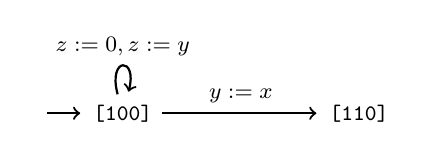
\begin{tikzpicture}
[
  highlight/.style={draw=blue, text=blue},
  shorten >=1pt,
  node distance=2cm,
  on grid,
  auto,
  /tikz/initial text={},
  font=\footnotesize,
  thick
]
 \node[rectangle,thick,initial left,draw=none] (l0) {\texttt{[100]}};
 \node[rectangle,thick,draw=none] (l1) [right=3cm of l0] {\texttt{[110]}};

  \path[->] 
    (l0) edge [thick,loop above] node [above] {$z := 0, z := y$} (l0)
    (l0) edge [thick] node [above] {$y := x$} (l1);
\end{tikzpicture}
}
\end{center}
From state \verb'[110]', executing $z := 0$ or $y := x$ leaves the taint mapping the same, but executing $z := y$ would result in \verb'[111]'. However, $z$ is a sink variable so entering this state would be a policy violation, and we leave the edge out.
\begin{center}
\scalebox{1.2}{%
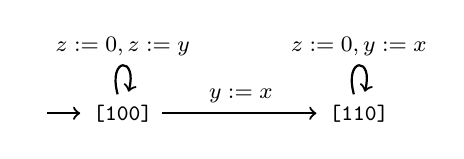
\begin{tikzpicture}
[
  highlight/.style={draw=blue, text=blue},
  shorten >=1pt,
  node distance=2cm,
  on grid,
  auto,
  /tikz/initial text={},
  font=\footnotesize,
  thick
]
 \node[rectangle,thick,initial left,draw=none] (l0) {\texttt{[100]}};
 \node[rectangle,thick,draw=none] (l1) [right=3cm of l0] {\texttt{[110]}};

  \path[->] 
    (l0) edge [thick,loop above] node [above] {$z := 0, z := y$} (l0)
    (l0) edge [thick] node [above] {$y := x$} (l1)
    (l1) edge [thick,loop above] node [above] {$z := 0, y := x$} (l1);
\end{tikzpicture}
}
\end{center}
The full automaton has additional states and transitions. For example, if the taint mapping were \verb'[010]', then executing $y := x$ would transition to \verb'[000]', whereas executing $z := 0$ would stay in the same state. Moreover, executing any instruction in \verb'[000]' stays in that state, so we would add this to the automaton.
\begin{center}
\scalebox{1.2}{%
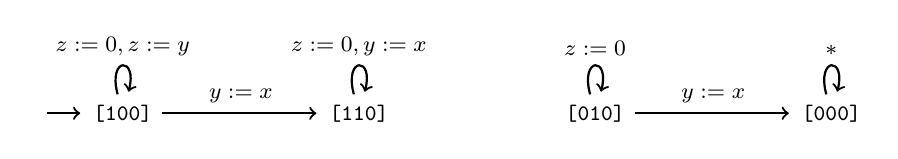
\begin{tikzpicture}
[
  highlight/.style={draw=blue, text=blue},
  shorten >=1pt,
  node distance=2cm,
  on grid,
  auto,
  /tikz/initial text={},
  font=\footnotesize,
  thick
]
 \node[rectangle,thick,initial left,draw=none] (l0) {\texttt{[100]}};
 \node[rectangle,thick,draw=none] (l1) [right=3cm of l0] {\texttt{[110]}};
 \node[rectangle,thick,draw=none] (l2) [right=3cm of l1] {\texttt{[010]}};
 \node[rectangle,thick,draw=none] (l3) [right=3cm of l2] {\texttt{[000]}};

  \path[->] 
    (l0) edge [thick,loop above] node [above] {$z := 0, z := y$} (l0)
    (l0) edge [thick] node [above] {$y := x$} (l1)
    (l1) edge [thick,loop above] node [above] {$z := 0, y := x$} (l1)
    (l2) edge [thick] node [above] {$y := x$} (l3)
    (l2) edge [thick,loop above] node [above] {$z := 0$} (l2)
    (l3) edge [thick,loop above] node [above] {$\mathtt{*}$} (l3);
\end{tikzpicture}
}
\end{center}
But these states are not reachable from the initial state of the SA, so we can leave them out and stop here.

\paragraph{Implicit flows.} So far taint analysis seems to do what we want in terms of tracking information flow as the program executes. So why did we say that it is an approximation of information flow, and moreover, why doesn't this contradict our thought experiment from earlier?

Recall that the program $\asprg_1$ in (\ref{eq:flowexp}) flowed information from $x$ to $y$, effectively computing $y = (1 - x)$. But it did not compute this using an assignment with $x$ on the right hand side, and rather with a conditional statement and constant assignments in either branch. This is known as an \emph{implicit flow} because the information moves from $x$ to $y$ indirectly by the choice of which program to execute within the conditional, rather than explicitly via an assignment statement.

The taint analysis policy that we described doesn't deal with implicit flows because it only propagates taintedness through explicit assignments. In this way taint analysis \emph{underapproximates} information flow. Whenever taint analysis deems that information has flowed from a source to a sink, then an information flow exists in the program. But if it fails to identify a flow, then we can't conclude that there isn't one in the program because there could yet be an implicit flow.

Can we change the security automaton policy to account for implicit flows? Suppose that we added an additional mapping to the policy state, intuitively corresponding to whether the program counter is tainted. We'll denote this $\taint(\pc)$, and we want to make sure that it is set to 1 whenever a conditional statement on a tainted expression is executed. So for example, if $x$ is a source in program (\ref{eq:implicit1}) below, then the policy will be in a state where $\taint(\pc)=1$ after executing the instruction at \keywordfont{1}.
\begin{equation}
\label{eq:implicit1}
\begin{array}{ll}
\mathtt{1:} & \pifjump{x \ne 0}{4} \\
\mathtt{2:} & y := 0 \\
\mathtt{3:} & \pifjump{\mathtt{true}}{5} \\
\mathtt{4:} & y := 1 \\
\mathtt{5:} & \ldots
\end{array}
\end{equation}
Then we can adapt the policy so that whenever $\taint(\pc) = 1$ in the current state, the target of \emph{any} assignment will become tainted. In (\ref{eq:implicit1}), this will ensure that $y$ is tainted after the conditional at \keywordfont{1}, and thus reflect the fact that there is an information flow from $x$ to $y$ in the program.

But now consider what happens if we add another instruction, as in (\ref{eq:implicit2}).
\begin{equation}
\label{eq:implicit2}
\begin{array}{ll}
\mathtt{1:} & \pifjump{x \ne 0}{3} \\
\mathtt{2:} & y := 0 \\
\mathtt{3:} & \pifjump{\mathtt{true}}{5} \\
\mathtt{4:} & y := 1 \\
\mathtt{5:} & z := 0
\end{array}
\end{equation}
Now under the current policy, $z$ will become tainted because it is executed after the tainted conditional. But there is clearly no flow of information from $x$ to $z$, so the taint mapping no longer reflects the actual flows in the program. Perhaps we could refine the policy further, by un-tainting the program counter once control returns to instructions that are in no way conditional on tainted data. In (\ref{eq:implicit2}), this is true for the assignment to $z$ at instruction \keywordfont{5} because it is executed regardless of the condition at \keywordfont{1}.

But how do we identify instructions that aren't conditional on tainted data in general? It was easy in this program, but things could get much more complicated as shown in (\ref{eq:implicit3}).
\begin{equation}
\label{eq:implicit3}
\begin{array}{ll}
\mathtt{1:} & \pifjump{x \ne 0}{6} \\
\mathtt{2:} & y := 0 \\
\mathtt{3:} & \pifjump{\precv\mathtt{()} \ne 0}{7} \\
\mathtt{4:} & \pifjump{\mathtt{true}}{6} \\
\mathtt{5:} & y := 1 \\
\mathtt{6:} & z := 0 \\
\mathtt{7:} & \ldots
\end{array}
\end{equation}
Now in order to tell whether to untaint the program counter before executing instruction 6, we need to predict the outcome of a network read. This policy has gotten significantly more complicated, and keep in mind that we need to do all of these calculations at runtime, which may impose considerable overhead on the target program.

Finally, even if we could solve this problem, tracking taint across implicit flows still may not accurately reflect a program's information flows. Consider the program in (\ref{eq:implicit4}) below.
\begin{equation}
\label{eq:implicit4}
\begin{array}{ll}
\mathtt{1:} & \pifjump{x \ne 0}{3} \\
\mathtt{2:} & y := 0 \\
\mathtt{3:} & \pifjump{\mathtt{true}}{5} \\
\mathtt{4:} & y := \mathtt{complicated\_function()} \\
\mathtt{5:} & \ldots
\end{array}
\end{equation}
It may turn out that $\mathtt{complicated\_function()}$ always returns 0, so that $y$ always takes the same value after the conditional regardless of what $x$ is. In this case, there is no real flow of information from $x$ to $y$. But our security automaton policy can't reason this way, because it would require considering a different trace from the one that was actually executed. Even if it could, it would need to reason about the behavior of an arbitrarily complicated, possibly non-terminating function, which is clearly not possible.

\section{Formalizing information flow: Non-interference}

We will now turn to a precise formalization of information flow properties in terms of \emph{non-interference}~\cite{Goguen1984}. We will see how non-interference can be proved using the axioms of dynamic logic, and eventually our goal will be to design a type system that ensures well-typed programs satisfy non-interference. But first we'll introduce some preliminaries that make the definition more clear, and return to the simple imperative language that we started with earlier in the semester.
\begin{equation*}
  \asprg,\bsprg ~\bebecomes~
  \pupdate{\pumod{x}{\astrm}}
  \alternative
  \passert{\ivr}
  \alternative
  \pif{\ivr}{\asprg}{\bsprg}
  \alternative
  \asprg;\bsprg
  \alternative
  \pwhile{\ivr}{\asprg}
\end{equation*}
Recall that states in this language are mappings from variables to values. Previously we studied the trace semantics of this language. For the purposes of introducing non-interference, it is helpful to now introduce the \emph{big-step transition relation} $\bigstep$. Given a program $\asprg$ and state $\omega$, we write:
\begin{equation}
\langle \omega, \asprg\rangle \bigstep \omega'
\end{equation}
to denote the fact that by executing $\asprg$ starting in $\omega$ it is possible to terminate in state $\omega'$. We can define a similar relation for terms and write $\langle \omega, \astrm\rangle \bigstep_e v$ to denote the fact that evaluating term $\astrm$ in $\omega$ gives value $v$. In the next lecture, we will define these relations in full detail, but for now understanding what they represent is sufficient.

\paragraph{Information flow policies.}
We will now make use of an information flow policy $\Gamma$ that maps each variable to a security label \lowsec or \hisec, for low or high security, respectively. We'll write specific policies out as lists, so the policy that maps $x$ to \lowsec and $y$ to \hisec is $(x:\lowsec, y:\hisec)$. If $\Gamma$ is a policy, possibly containing a mapping for $x$, then $(\Gamma, x:\lowsec)$ is the policy that treats $x$ as \lowsec and everything else $y$ as $\Gamma(y)$.

Let $\omega_1$ and $\omega_2$ be states, and $\Gamma$ be a policy. Then we say that $\omega_1$ and $\omega_2$ are $\ell$-equivalent, where $\ell \in \{\lowsec,\hisec\}$ is a security label, if and only if all of the variables where $\Gamma(x) = \ell$ have the same value in $\omega_1$ and $\omega_2$.
\begin{equation}
\label{eq:secequiv}
\forall x . \Gamma(x) = \ell \limply \omega_1(x) = \omega_2(x)
\end{equation}
We use the notation $\omega_1 \approx_{\Gamma,\ell} \omega_2$ to denote the relation in Equation~\ref{eq:secequiv}, and if the choice of $\Gamma$ is clear from the context, we will abbreviate it as $\omega_1 \approx_{\ell} \omega_2$.

\subsection{Information flow as influence}
Now we can proceed with the formal definition. 

\begin{definition}[Non-interference]
\label{def:nonint}
Let $\asprg$ be a program and $\Gamma$ a policy associating security labels to all of the variables in $\asprg$. Then $\asprg$ satisfies non-interference under $\Gamma$ if and only if executing $\asprg$ under \lowsec-equivalent states leads to final states that are also \lowsec-equivalent. More precisely,
\begin{equation}
\label{eq:noninterference}
\forall \omega_1,\omega_2 . \omega_1 \approx_{\Gamma,\lowsec} \omega_2 \land 
\langle \omega_1, \asprg\rangle \bigstep \omega_1' \land 
\langle \omega_2, \asprg\rangle \bigstep \omega_2'
\limply
\omega_1' \approx_{\Gamma,\lowsec} \omega_2'
\end{equation}
where $\omega_1$ and $\omega_2$ range over the set of possible program states.
\end{definition}

Equation~\ref{eq:noninterference} captures the idea that whatever the values of variables labeled \hisec may be, they should not influence the values that the \lowsec variables take when the program terminates. If such influence exists, then the program does \emph{not} satisfy non-interference. In this way, non-interference equates information flow with the tendency of one variable to influence another.

Let's now return to some of the programs we've discussed today, and apply Definition~\ref{def:nonint} to build our intuition. Recalling $\asprg_1$ from (\ref{eq:flowexp}),
\[
\asprg_1 \equiv x := x; \pif{x = 1}{y:=0}{y:=1}
\]
We've stated informally that this program has an information flow from $x$ to $y$. The corresponding policy that we would assign to reason about the corresponding instance of non-interference is $\Gamma = (x : \hisec, y : \lowsec)$. Now, to satisfy non-interference, it must be that for all \lowsec-equivalent initial states, i.e. those that agree on the value of $y$, the final states must also be \lowsec-equivalent. In other words, regardless of how we assign $x$ at the beginning, whatever value $y$ took should remain in the end.

We already reasoned in the thought experiment that if $\omega_1(x) = 0$ and $\omega_2(x) = 1$ and $\omega_1(y) = \omega_2(y) = 0$, then,
\[
\begin{array}{ll}
\langle \omega_1, \asprg\rangle \bigstep \omega_1', & \text{and}~\omega_1'(y) = 1 \\
\langle \omega_2, \asprg\rangle \bigstep \omega_2', & \text{and}~\omega_2'(y) = 0 \\
\end{array}
\]
So these initial states $\omega_1,\omega_2$ serve as a counterexample to Equation~\ref{eq:noninterference}, and we conclude that this program does not satisfy non-interference. On the other hand if we modified the program slightly so that $y$ took the same value on both branches,
\[
\asprg \equiv x := x; \pif{x = 1}{y:=0}{y:=0}
\]
then we would not be able to find such a counterexample, and we would conclude that $\asprg$ satisfies non-interference.

\paragraph{Proving non-interference.}
How might we prove that a program satisfies Definition~\ref{def:nonint}? As Terauchi and Aiken~\cite{Terauchi2005} reasoned, although non-interference of $\asprg$ is not a safety property of $\asprg$, one can find a different program $\bsprg$ and safety property such that the property holds on $\bsprg$ if and only if $\asprg$ satisfies non-interference.

They observed that while safety properties are defined over one trace of a program, non-interference can be defined over pairs of traces. This is apparent in Definition~\ref{def:nonint}, where $\omega_1$ and $\omega_2$ naturally correspond to two distinct traces of $\asprg$ whose initial states agree on variables labeled \lowsec. Moreover, we can obtain a program whose traces correspond to pairs of $\asprg$'s traces by a simple trick. Namely, if we make a copy $\asprg'$ of $\asprg$ and ensure that all of its variables are distinct from $\asprg$, e.g. by suffixing a prime character to each variable name, then one trace of $\asprg;\asprg'$ corresponds to a pair of traces of $\asprg$.

This is best illustrated with an example. Suppose that our program $\asprg$ is given in (\ref{eq:selfcomp1})
\begin{equation}
\label{eq:selfcomp1}
x := x + 1; y := x; z := y
\end{equation}
Then we obtain a copy $\asprg'$ by priming the variables in (\ref{eq:selfcomp2})
\begin{equation}
\label{eq:selfcomp2}
x' := x' + 1; y' := x'; z' := y'
\end{equation}
The \emph{self-composed} program $\asprg;\asprg'$ is then shown in (\ref{eq:selfcomp3})
\begin{equation}
\label{eq:selfcomp3}
x := x + 1; y := x; z := y; x' := x' + 1; y' := x'; z' := y'
\end{equation}
Any trace of (\ref{eq:selfcomp3}) can be decomposed into two traces of $\asprg$. But note that if we had not made the variables in $\asprg'$ distinct from those in $\asprg$,
\begin{equation}
\label{eq:selfcomp4}
x := x + 1; y := x; z := y; x := x + 1; y := x; z := y
\end{equation}
Then we no longer have this property, because after the first part is finished executing, $\asprg'$ picks up on the same state and modifies it in a way that could never have happened in the original program.

Having obtained a self-composed $\asprg;\asprg'$, we can reason about non-interference by assuming that all of the variables labeled \lowsec begin with the same values in their unprimed and primed versions. We then require that when $\asprg;\asprg'$ finishes executing, the primed and unprimed \lowsec variables still have matching values.
\begin{equation}
\label{eq:selfcompex}
\lsequent{\forall x . \Gamma(x) = \lowsec \limply x = x'}{\dbox{\asprg;\asprg'}{(\forall x . \Gamma(x) = \lowsec \limply x = x'})}
\end{equation}
For example, applying this to (\ref{eq:selfcomp3}) we would construct a proof of the following under $\Gamma = (x : \hisec, y : \lowsec, z : \lowsec)$.
\begin{equation}
\lsequent{y = y', z = z'}{\dbox{\asprg;\asprg'}{y = y' \land z = z'}}
\end{equation}
Of course, we will not be able to construct such a proof, as the original $\asprg$ in (\ref{eq:selfcomp1}) does not satisfy non-interference under this policy.

\bibliographystyle{abbrv}
\bibliography{bibliography}
\end{document}